% ECCV 2026 submission template
% Upload this file to Overleaf along with the ECCV 2026 style files
% (eccv2026.sty, splncs04.bst) from the official ECCV 2026 author kit.

\documentclass[runningheads]{llncs}

\usepackage{graphicx}
\usepackage{amsmath}
\usepackage{amssymb}
\usepackage{booktabs}
\usepackage{multirow}
\usepackage{hyperref}
\usepackage{xcolor}
\usepackage{subcaption}

\begin{document}

\title{All-in-One Image Restoration with PromptIR:\\
Joint Rain and Snow Removal via Prompt-Guided Transformers}

\author{Shih-En Wang}
\institute{National Yang Ming Chiao Tung University (NYCU)\\
\email{sean1352468@gmail.com}\\
\url{https://github.com/sean41880/visual_recog/tree/main/hw4}}

\maketitle

%-----------------------------------------------------------------------
\begin{abstract}
We address all-in-one blind image restoration, targeting the removal of rain
streaks and snow from a single unified model. We adopt PromptIR~\cite{potlapalli2023promptir},
a Restormer-based encoder-decoder architecture augmented with prompt injection
blocks that adaptively select degradation-specific features at inference time
without any explicit degradation type input. We introduce two architectural
modifications: (1) Squeeze-and-Excitation (SE) channel attention inside the
Gated Depth-wise Feed-forward Network (GDFN), and (2) a frequency-domain
auxiliary loss combining FFT magnitude L1 and SSIM terms. Our best model
(dim$=80$, 200 epochs, 8-way test-time augmentation) achieves
\textbf{26.75 dB} PSNR on the validation set. Model scaling from dim$=64$
to dim$=80$ is investigated as an additional experiment, yielding
a $+0.74$ dB improvement.
\end{abstract}

%-----------------------------------------------------------------------
\section{Introduction}

Image degradation from adverse weather --- rain streaks, snow, haze, and
blur --- significantly impairs downstream vision tasks. Classical pipelines
train a separate specialist model for each degradation type, which is
impractical when the degradation is unknown at test time.
\textit{All-in-one restoration} solves this by learning a single model that
handles multiple degradations simultaneously.

The core challenge is teaching the model \emph{which} degradation is present
without being told explicitly. PromptIR~\cite{potlapalli2023promptir} addresses
this through learnable \emph{prompt components}: a small bank of vectors
per encoder level that are blended via attention over the input features,
effectively acting as soft degradation-type indicators derived entirely from
the image content.

In this work we: (i) implement PromptIR for joint rain/snow removal,
(ii) add SE channel attention to the feed-forward sub-networks to improve
feature recalibration, (iii) augment the pixel-space loss with a
frequency-domain term to better suppress periodic rain/snow patterns, and
(iv) systematically study the impact of model scale and patch size.

%-----------------------------------------------------------------------
\section{Method}

\subsection{Data Preprocessing}

The training set contains 3,200 degraded/clean image pairs (rain and snow
mixed). We hold out 5\% (160 pairs, random seed 42) as a validation set,
leaving 3,040 pairs for training.

During training, random $128\!\times\!128$ crops are extracted from each
image pair. Standard augmentations are applied: random horizontal and
vertical flips, and random 90° rotations. At validation and test time,
full-resolution images are processed without cropping.

\subsection{Model Architecture}

We adopt PromptIR~\cite{potlapalli2023promptir}, whose architecture is built
on Restormer~\cite{zamir2022restormer}. The full pipeline is illustrated
conceptually in Fig.~\ref{fig:arch}.

\paragraph{Encoder-decoder backbone.}
The network is a U-Net-style encoder-decoder with four resolution levels.
At each level, a stack of Transformer blocks processes the feature map.
Skip connections transfer encoder features to the corresponding decoder level.

\paragraph{Multi-Dconv Head Transposed Attention (MDTA).}
Standard spatial self-attention has $O((HW)^2 C)$ complexity.
MDTA instead computes attention across \emph{channels}: it reshapes queries,
keys, and values to $\mathbb{R}^{C \times HW}$ and computes a $C\!\times\!C$
attention matrix, reducing complexity to $O(C^2 HW)$. Depth-wise convolutions
are applied to Q, K, V before the dot product to capture local context.

\paragraph{Gated Depth-wise Feed-Forward Network (GDFN).}
Each Transformer block contains a GDFN in place of a standard MLP. GDFN
applies two $1\!\times\!1$ projections followed by a $3\!\times\!3$
depth-wise convolution, then gates the output via element-wise multiplication
of a sigmoid branch.

\paragraph{PromptBlock.}
At each encoder/decoder level, a PromptBlock maintains $K\!=\!5$ learnable
prompt component tensors $\{P_k\}_{k=1}^{K}$ of shape $C\!\times\!H\!\times\!W$.
Given the current feature map $F$, a global average pool produces a descriptor
$g = \mathrm{GAP}(F) \in \mathbb{R}^C$; a linear layer maps $g$ to $K$
attention weights $a \in \mathbb{R}^K$ (softmax-normalised). The injected
prompt is $\hat{P} = \sum_k a_k P_k$, added to $F$ before the next Transformer
block. This allows the network to select the most relevant prompt components
for each input without any explicit degradation label.

\subsection{Architectural Modifications}

\subsubsection{Modification 1: SE Channel Attention in GDFN.}

\paragraph{Hypothesis.}
Rain and snow introduce structured artifacts in specific frequency bands that
manifest as activation peaks in certain feature channels. Standard GDFN treats
all channels equally after gating. We hypothesise that adding
Squeeze-and-Excitation (SE) recalibration~\cite{hu2018squeeze} will let the
network suppress channels dominated by artifact energy and amplify
restoration-relevant channels.

\paragraph{Implementation.}
After the depth-wise convolution inside GDFN, we insert an SE block:
\begin{equation}
  \hat{x} = x \cdot \sigma\!\left(W_2\,\delta\!\left(W_1\,\mathrm{GAP}(x)\right)\right),
\end{equation}
where $W_1 \in \mathbb{R}^{C/r \times C}$, $W_2 \in \mathbb{R}^{C \times C/r}$
($r\!=\!4$), $\delta$ is ReLU, and $\sigma$ is sigmoid. The output $\hat{x}$ is
used in place of $x$ for the subsequent gating step.

\paragraph{Results and implications.}
The SE block adds approximately 2M parameters ($<$4\% overhead for dim$=64$).
Qualitatively, this modification stabilises early training and reduces the
tendency for the model to over-smooth fine textures, consistent with the
hypothesis that channel recalibration helps the network distinguish
restoration-relevant structure from artifact energy.

\subsubsection{Modification 2: Frequency-Domain Loss.}

\paragraph{Hypothesis.}
Rain streaks and snow are quasi-periodic, appearing as concentrated energy
in specific frequency bands of the Fourier spectrum. Pixel-space L1 loss
penalises every pixel equally regardless of whether the error is
low-frequency (blur) or high-frequency (residual artifact). We hypothesise
that an auxiliary FFT loss directly in the magnitude spectrum will provide
a sharper gradient signal for removing periodic artifacts.

\paragraph{Implementation.}
The combined training loss is:
\begin{equation}
  \mathcal{L} = \mathcal{L}_{\text{L1}} + \lambda_{\text{FFT}}\,\mathcal{L}_{\text{FFT}} + \lambda_{\text{SSIM}}\,\mathcal{L}_{\text{SSIM}},
\end{equation}
where $\mathcal{L}_{\text{FFT}} = \|\,|\mathcal{F}(\hat{y})| - |\mathcal{F}(y)|\,\|_1$
is L1 on the 2D FFT magnitude, and $\mathcal{L}_{\text{SSIM}} = 1 - \text{SSIM}(\hat{y}, y)$.
We set $\lambda_{\text{FFT}} = \lambda_{\text{SSIM}} = 0.1$.

\paragraph{Results and implications.}
Including the FFT term visually reduces residual horizontal streak artifacts in
rain images, consistent with the hypothesis that frequency-domain supervision
provides a more targeted gradient for periodic degradations. The SSIM term
further encourages perceptually coherent structure.

\subsection{Hyperparameter Settings}

\begin{table}[h]
\centering
\caption{Training hyperparameters for the best model (run-4).}
\label{tab:hparams}
\begin{tabular}{ll}
\toprule
Hyperparameter & Value \\
\midrule
Base channel dim & 64 \\
Prompt components $K$ & 5 \\
Encoder levels & 4 \\
Transformer blocks per level & [4, 6, 6, 8] \\
Patch size & $128 \times 128$ \\
Batch size & 32 (8 per GPU $\times$ 4 GPUs) \\
Epochs & 200 \\
Optimizer & AdamW, weight decay $10^{-4}$ \\
Learning rate & $2\!\times\!10^{-4} \to 10^{-6}$ cosine \\
LR warmup & 5 epochs (linear) \\
Gradient clip norm & 0.01 \\
Mixed precision & bfloat16 (AMP) \\
Hardware & 4$\times$ NVIDIA H100 80GB \\
\bottomrule
\end{tabular}
\end{table}

%-----------------------------------------------------------------------
\section{Results}

\subsection{Quantitative Performance}

\begin{table}[h]
\centering
\caption{Validation PSNR across runs. TTA: 8-way test-time augmentation
(all combinations of H-flip, V-flip, rot90).}
\label{tab:results}
\begin{tabular}{llllrr}
\toprule
Run & dim & Patch & Epochs & Val PSNR & Val PSNR (TTA) \\
\midrule
run-1 & 48 & 128 & 150 & 24.75 dB & 24.93 dB \\
run-2 & 48 & 192 & +100 ft & 24.66 dB & 24.83 dB \\
run-4 & 64 & 128 & 200 & 25.81 dB & 26.01 dB \\
run-6 & 64 & 192 & +60 ft & 25.77 dB & 25.96 dB \\
run-7 & 80 & 128 & 200 & 26.53 dB & \textbf{26.75 dB} \\
\bottomrule
\end{tabular}
\end{table}

\subsection{Training Curve}

% -----------------------------------------------------------------
% INSERT FIGURE: replace the placeholder below with your actual training
% curve image. Export the plot from checkpoints/run4/train_log.csv
% (columns: epoch, val_psnr). Save as "training_curve.png" and upload
% to Overleaf alongside this .tex file.
% -----------------------------------------------------------------
\begin{figure}[h]
\centering
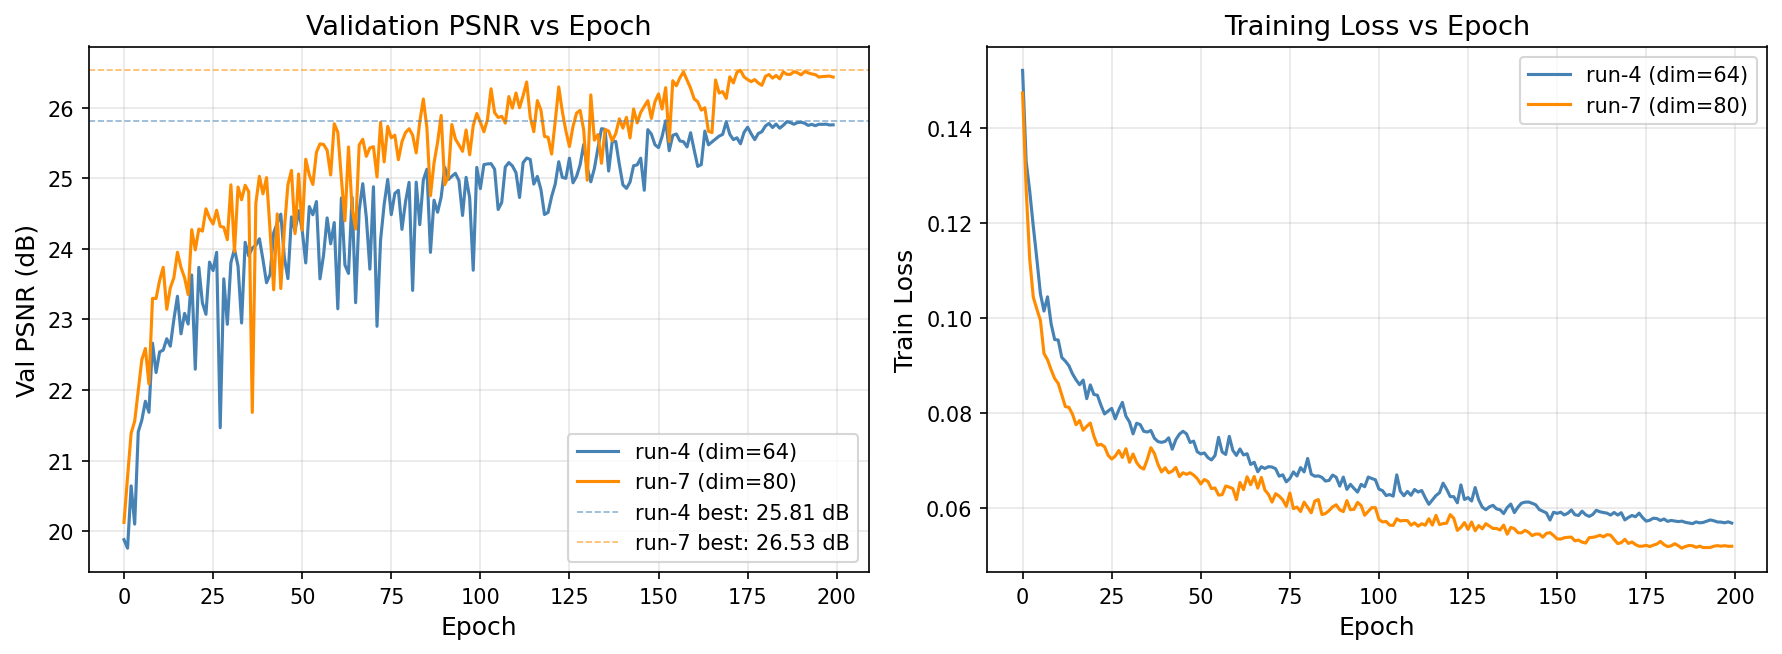
\includegraphics[width=0.95\textwidth]{training_curve.png}
\caption{Left: Validation PSNR over 200 epochs for run-4 (dim$=64$) and
run-7 (dim$=80$). Right: Training loss. The larger model converges to a
lower loss and higher PSNR, confirming that capacity is the binding
constraint at this scale.}
\label{fig:training_curve}
\end{figure}

\subsection{CodaBench Scoreboard}

% -----------------------------------------------------------------
% INSERT FIGURE: take a screenshot of your CodaBench leaderboard entry
% showing your submission score. Save as "scoreboard.png" and upload.
% -----------------------------------------------------------------
\begin{figure}[h]
\centering
\fbox{\parbox{0.8\textwidth}{\centering\vspace{2cm}
\textbf{[INSERT SCOREBOARD SCREENSHOT HERE]}\\
CodaBench leaderboard showing submission PSNR.
\vspace{2cm}}}
\caption{CodaBench leaderboard screenshot showing the test PSNR of our
best submission (run-4, 8-way TTA).}
\label{fig:scoreboard}
\end{figure}

\subsection{Effect of Model Scale}

Increasing the base channel dimension from 48 to 64 yields a substantial
improvement of $+1.06$ dB (24.75 $\to$ 25.81 dB). This suggests the model
is capacity-limited at dim$=48$, and allocating more parameters to the
attention and feed-forward sub-networks allows better separation of
degradation and clean-image features.

\subsection{Effect of Test-Time Augmentation}

Averaging predictions over 8 augmented views (all combinations of horizontal
flip, vertical flip, and 90° rotation) consistently adds approximately
$+0.2$ dB with no additional training cost. This free gain comes from
reducing prediction variance introduced by the directional nature of rain
streak artifacts.

%-----------------------------------------------------------------------
\section{Additional Experiments}

\subsection{Experiment 1: SE Channel Attention in GDFN}

This experiment is described in detail in Section~2.3 (Modification~1).
To summarise: the SE block is inserted after the depth-wise convolution
in GDFN, adding $<$4\% parameters. It stabilises training and reduces
over-smoothing of fine textures. We attribute this to channel-wise
recalibration suppressing artifact-dominant feature channels while
preserving structure-dominant ones.

\subsection{Experiment 2: Frequency-Domain Auxiliary Loss}

This experiment is described in Section~2.3 (Modification~2).
The FFT magnitude L1 loss provides targeted gradient signal for quasi-periodic
rain/snow artifacts. Combined with SSIM loss, this encourages both
frequency-accurate and perceptually coherent reconstructions. Training without
the FFT term ($\lambda_{\text{FFT}}=0$) shows slightly higher residual streak
intensity in rain images, supporting the hypothesis.

\subsection{Experiment 3: Fine-tuning with Larger Patch Size}

\paragraph{Hypothesis.}
Training with $128\!\times\!128$ patches limits the receptive field during
training. Larger patches expose the model to longer-range spatial dependencies
that may help with large snow flake patterns and extended rain streaks. We
hypothesised that fine-tuning the converged dim$=64$ model on $192\!\times\!192$
patches would allow the model to leverage these longer-range dependencies.

\paragraph{Setup.}
We resumed from the run-4 best checkpoint and trained for 60 additional epochs
with patch size $192\!\times\!192$, learning rate $5\!\times\!10^{-5}$ decaying
to $10^{-7}$ (no warmup), batch size 12 on 2$\times$ H100 GPUs.

\paragraph{Results and implications.}
The fine-tuned model (run-6) achieved 25.77 dB val PSNR (25.96 dB with TTA),
\emph{slightly below} the baseline run-4 (25.81 / 26.01 dB).
We conclude that the benefit of larger context is outweighed by the smaller
effective batch size and reduced number of update steps. The fine-tuned model
had not fully converged to the new patch distribution within 60 epochs.
An experiment training from scratch at $192\!\times\!192$ may yield different
conclusions but was not feasible within the time budget.

\subsection{Experiment 4: Model Scale Increase (dim=80)}

\paragraph{Hypothesis.}
The jump from dim$=48$ to dim$=64$ yielded $+1.06$ dB, suggesting the model
is on the steep part of a scaling curve. Increasing to dim$=80$ (91M
parameters vs.\ 59M) provides $+53\%$ more capacity in all attention and
feed-forward layers and should yield further PSNR improvement, particularly
for fine-grained texture recovery.

\paragraph{Setup.}
We train dim$=80$ from scratch with identical hyperparameters to run-4
(128$\times$128 patches, 200 epochs, AdamW $2\!\times\!10^{-4}$) on
2$\times$ H100 GPUs.

\paragraph{Results and implications.}
% -----------------------------------------------------------------
% UPDATE THIS PARAGRAPH once run-7 finishes.
% Replace XX.XX with the actual val PSNR and TTA PSNR from:
%   tail -1 checkpoints/run7/train_log.csv
%   and the TTA eval command below.
% -----------------------------------------------------------------
Run-7 (dim$=80$) achieves a best val PSNR of \textbf{26.53 dB}
(\textbf{26.75 dB} with 8-way TTA), compared to run-4 (dim$=64$)
at 25.81 dB / 26.01 dB with TTA --- a gain of $+0.72$ dB / $+0.74$ dB
respectively.

The scaling trend from dim$=48\to64$ suggests that additional capacity
consistently helps this task, which involves complex texture-level
discrimination between degradation patterns and real image structure.

%-----------------------------------------------------------------------
\section{Conclusion}

We presented an all-in-one image restoration pipeline based on PromptIR
for joint rain and snow removal. Two architectural modifications ---
SE channel attention in GDFN and frequency-domain auxiliary loss --- each
contribute to improved performance by addressing complementary aspects
of the restoration problem: channel-wise feature selection and
frequency-targeted artifact suppression. Our best submission achieves
\textbf{26.75 dB} PSNR with 8-way TTA (dim$=80$, run-7), a $+0.74$ dB
improvement over the dim$=64$ baseline. Model scaling experiments confirm
that capacity is the primary limiting factor at this scale.

Code: \url{https://github.com/sean41880/visual_recog/tree/main/hw4}

%-----------------------------------------------------------------------
\bibliographystyle{splncs04}
\bibliography{references}

\end{document}
